%Dokumententyp
\documentclass[a4paper]{article}

\usepackage[a4paper,left=2cm, right=3cm, top=2cm]{geometry}

%Kodierung
\usepackage[utf8]{inputenc}
\usepackage[T1]{fontenc}

%Grafiken einbinden
\usepackage{graphicx}
\usepackage{subfigure} 

%Position von Grafiken und Tabellen erzwingen:
\usepackage{float}

%URLs im Literaturverzeichnis
\usepackage{url}

\usepackage{amsmath}

%Vektoren einfacher angeben:
\newcommand{\vektor}[1]{\left( \begin{array}{c} #1 \end{array} \right) }


%Schriftart Arial:
% \usepackage{helvet}

%Figures with text around it:
\usepackage{wrapfig}

\usepackage{listings}

%seitennummern rechts:
% \usepackage{fancyhdr}
% \fancyhf{} % clear all header and footers
% \renewcommand{\headrulewidth}{0pt} % remove the header rule
% \rfoot{\thepage}
% \fancypagestyle{plain}{%redefining plain pagestyle
% \fancyhf %clear all headers and footers fields
% \fancyhead[R]{\thepage} %prints the page number on the right side of the header
% }

%Schriftart Times New Roman "like"
\usepackage{txfonts}

%Sprache
\usepackage[german]{babel}

%Checkmarks: (usage: \checkmark)
\usepackage{dingbat}

\usepackage{listings}
\usepackage{color}
\definecolor{javared}{rgb}{0.6,0,0} % for strings
\definecolor{javagreen}{rgb}{0.25,0.5,0.35} % comments
\definecolor{javapurple}{rgb}{0.5,0,0.35} % keywords
\definecolor{javadocblue}{rgb}{0.25,0.35,0.75} % javadoc
 
\lstset{language=Java,
basicstyle=\ttfamily,
keywordstyle=\color{javapurple}\bfseries,
stringstyle=\color{javared},
commentstyle=\color{javagreen},
morecomment=[s][\color{javadocblue}]{/**}{*/},
numbers=left,
numberstyle=\tiny\color{black},
stepnumber=1,
numbersep=5pt,
tabsize=4,
showspaces=false,
lineskip={-1.5pt},
showstringspaces=false}

%Tabellenextras
\usepackage{tabularx}

% Gradzeichen..:)
\usepackage{textcomp}

%Zeilenabstand 1.5
\linespread{1.5}
\usepackage{setspace}

%URLs
\usepackage{url}

%
\usepackage{cancel}

%Figure Captions mit Fußnoten
\usepackage{footnote}
%\setlength{\parindent}{0pt} 

%Graphen/Trees zeichnen:
\usepackage{tikz}
\newcommand*\circled[1]{\tikz[baseline=(char.base)]{
            \node[shape=circle,draw,inner sep=2pt] (char) {#1};}}


%itemize items richtig ausrichten (nicht links überlappen!)
% \setlist{leftmargin=0}

% %%%%TITELSEITE%%%%%%(
% \title{ Konzept und Implementierung\\ eines Systems zur \\Anforderung und Verwaltung von virtuellen privaten Clustern}
% \author{\textbf{\large Bachelorarbeit}}
% 
% \date{zur Erlangung des akademischen Grades Bachelor of Science an der Universität Paderborn im Fachbereich Informatik im Studiengang Bachelor Informatik}

% %%%%TITELSEITE%%%%%%)

% \pagestyle{fancy}
\begin{document}

\title{Algorithmische Geometrie - Sommersemester 2015\\
       11. Aufgabenblatt }
\author{Simon Koennecke und Felix Bröker}
\date{}
\maketitle

\section*{Aufgabe 1: Konfliktecken}


Gegeben ist eine Menge von Halbräumen $H = \{h_1, \dots, h_n\}$ mit $h_i \subset \mathcal{R}^3$ und $|H| = n$.
% Für alle Halbräume $h_i \in H$ und $h_j \in H$ gelte $h_i \cap h_j \neq h_i$ mit $i \neq j$.
Die einzelnen Halbräume $h_i \in H$ seien durch die hessesche Normalform für Ebenen 
repräsentiert, wobei der jeweilige Normalenvektor in die Richtung des spezifizierten
Halbraums zeigt. Des Weiteren gelte für alle zu zwei Halbräumen
$h_i, h_j \in H$ (entsprechend der Hesseschen Normalform) gehörenden Ebenen $e_i, e_j$ mit $i \neq j$, dass diese nicht parallel zueinander sind.


\begin{figure}[!htb]
\centering
\subfigure[Illustration des initialen Konfliktgraphen]{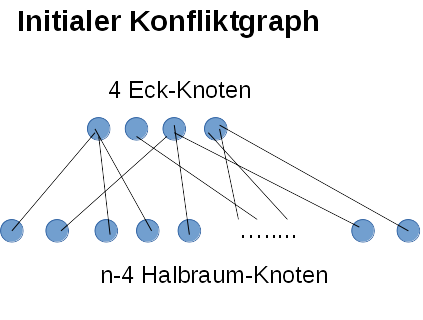
\includegraphics[width=0.35\textwidth]{konfliktgraph}} 
\end{figure} 



Zunächst nehmen wir vier Halbräume $h_i, h_j, h_k, h_l \in H$. 
Diese spannen ein Tetraeder $T$ auf. 

Für den Aufbau der Konfliktstruktur (bipartiter Graph) erstellen wir als erstes 
"`Halbraum"'-Knoten für einen jeden Halbraum $h_i \in H$. Dies benötigt $\mathcal{O}(n-4)$
Zeit.

Dann erstellen wir für jede der 4 Ecken $k_i \in T$ einen "`Eck"'-Knoten im Konfliktgraph
($\mathcal{O}(1)$).
Anschließend durchlaufen wir alle noch verbleibenden Halbräume $h_i \in H$ 
und prüfen jeweils für jeden "`Eck"'-Knoten mit Ecke $k_i$ , ob $k_i$ nicht im 
jeweiligen Halbraum $h_i$ liegt (Dies kann beispielsweise direkt über die Hessesche Normalform
in konstanter Zeit ausgewertet werden.). Wenn dies der Fall ist, fügen wir eine Kante $e$ in 
den Konfliktgraph ein, welche den "`Eck"'-Knoten von Ecke $k_i$ mit dem "`Halbraum"'-Knoten
von $h_i$ verbindet. 

Da wir insgesamt $4 * (n-4)$ Operationen jeweils konstanter Zeit haben, benötigen
wir hier ebenfalls $\mathcal{O}(n)$ Zeit.

Insgesamt können wir somit die Konfliktstruktur in $\mathcal{O}(n)$ Zeit auf die beschriebene Weise initialisieren.









\section*{Aufgabe 2: Randomisiert inkrementelle Konstruktionen}



\subsection*{(a) konvexe Hülle}



Es sei eine Punktmenge $P = \left\{p_1, \dots, p_n\right\} \subset \mathcal{R}^2$ mit $|P| = n$ in allgemeiner Lage gegeben. Sei zudem $S_i$ die konvexe Hülle der ersten $i$ aus $P$
entnommenen Punkte.

Wir entnehmen zunächst drei beliebige Punkte $p_i, p_j, p_k$ aus $P$ und aktualisieren
$P$ mit $P = P \setminus \{p_i, p_j, p_k\}$. Wegen der allgemeinen Lage  spannen $p_i, p_j, p_k$
ein Dreieck und damit zugleich die konvexe Hülle $S_3$ auf. 

Zur Bearbeitung der nächsten
$n-3$ Punkte aus $P$ berechnen wir weiterhin den Schwerpunkt $s$ von $S_3$.
Den Schwerpunkt $s$ zusammen mit dem von $s$ nach rechts ausgehenden Strahl, welcher parallel zur x-Achse verläuft,
verwenden wir im weiteren Verlauf als "`Bezugsrahmen"' für die Berechnung des eingeschlossenen Winkels $\alpha \in [0,360)$ (wie bei Polarkoordinaten).
Außerdem erstellen wir einen AVL-Baum $B$, welcher zu Beginn jedes $i$ten Schrittes alle Punkte der konvexen Hülle $S_{i-1}$ entsprechend
der Winkel $\alpha_i$ enthält. Das heißt, zu Beginn werden entsprechend initial die Punkte $p_i, p_j, p_k$ bzgl. des jeweiligen Winkels $\alpha_i$ 
in $B$ eingefügt ($\mathcal{O}(\log 3) = \mathcal{O}(1)$).

Im Folgenden beschreiben wir nun den inkrementellen Schritt jeweils für alle weiteren $n-3$ Punkte $p_i \in P$.
Dabei nutzen wir das in der Vorlesung vorgestellte Konzept der "`Kegel"', welche durch die Strahlen 
vom Schwerpunkt $s$ durch die aktuellen Punkte der konvexen Hülle definiert sind, aus.

\begin{enumerate}
 \item Führe eine Binärsuche in $B$ mit $winkel(p_i)$ durch. Wir erhalten einen Punkt $p_k$, welcher einer der beiden Punkte
 aus $S_{i-1}$ ist, welche den gesuchten Kegel definieren.
 \item Falls $winkel(p_i) < winkel(p_k)$, führe eine Vorgänger-Suche in $B$ mit $winkel(p_k)$ aus, ansonsten analog eine Nachfolger-Suche.
 Damit haben wir den zweiten Punkt $p_l \in S_{i-1}$ des gesuchten Kegels bestimmt. 
 
 \textit{Hinweis: Ist ein Nachfolger bzw. Vorgänger nicht vorhanden, entnehme entsprechend das Minimum bzw. Maximum aus $B$.}
 \item Nun prüfen wir für den neu hinzuzufügenden Punkt $p_i$, ob dieser sich außer- oder innerhalb von $S_{i-i}$ befindet. 
 Dies können wir überprüfen, indem wir testen, ob der Punkt (je nach Definition und Lage der Punkte $p_k$ und $p_l$ in $S_{i-1}$ zueinander) rechts oder links der durch $p_k$ und $p_l$ definierten Geraden befindet. 
 \item Gilt also $p_i \in S_{i-1}$, so setzen wir $S_i = S_{i-1}$ und fahren mit dem nächsten Punkt im Schritt 1 fort. 
 
 Im anderen Fall setzen wir ebenfalls $S_i = S_{i-1}$, führen jedoch auch zusätzlich folgende Schritte für jeweils "`beide Richtungen"' der konvexen Hülle $S_{i-1}$ für $p_m \in \{p_k, p_l\}$  aus:
 \begin{enumerate}
  \item Wir berechnen den Winkel $\beta$ der Strecken $\overline{p_i p_m}$ und $\overline{p_m p_{m+1}}$, wobei $p_{m+1} \in S_{i-1}$ der nächste Punkt auf der konvexen
  Hülle in entsprechender Richtung ist. Ist der "`potentielle Innenwinkel"' $\beta < 180$\textdegree, so sind wir für diese Richtung fertig
  und merken uns $p_m$.
  \item Gilt $\beta > 180$\textdegree, so entfernen wir $p_m$ aus $B$, setzen $S_i = S_i \setminus \{p_m\}$, setzen $p_m = p_{m+1}$ und fahren mit (a) fort.
 \end{enumerate}

 Für "`beide Richtungen"' kennen wir nun die beiden Punkte aus $S_{i-1}$, zwischen denen der neue Punkt $p_i$ in der konvexen Hülle
 eingefügt werden muss. Aktualisiere entsprechend $S_i$ mit $S_i = S_i \cup \{p_i\}$. 
 Füge außerdem $p_i$ mit $winkel(p_i)$ zu $B$ hinzu.
 Fahre nun mit dem nächsten Punkt in Schritt 1 fort.
\end{enumerate}


\subsection*{Laufzeit}
Da laut Tutorium für diese Aufgabe eigentlich keine Laufzeitanalyse vorgesehen war, beschränken wir uns hier nur auf eine grobe Abschätzung
der Gesamtlaufzeit $T(n)$:

\begin{itemize}
 \item Initialisieren von $B$, $s$ und $S_3$: $\mathcal{O}(1)$
 \item n-3 mal:
 \begin{itemize}
  \item Kegel und zugehörige Punkte $\in S_{i-1}$ bestimmen: $\mathcal{O}(\log n)$
  \item Prüfen, ob Punkt $p_i$ rechts bzw. links der beschriebenen Geraden liegt: $\mathcal{O}(1)$
  \item Falls $p_i$ außerhalb von $S_{i-1}$ für "`beide Richtungen"' (also 2 mal):
  \begin{itemize}
   \item Winkel berechnen + Vergleichen: $\mathcal{O}(1)$
   \item Falls Winkel nicht konvex:
   
    $S_i$ und $p_m$ aktualisieren ($\mathcal{O}(1)$) und "`$x$-mal"' diesen und vorherigen Schritt wiederholen bis Winkel konvex
  \end{itemize}

 \end{itemize}

\end{itemize}




\subsection*{(b) Voronoi-Diagramm}

  

\end{document}

